\chapter{Transformaciones de M\"obius}

\section{Transformaciones de M\"obius}
\begin{defi}
Una transformación de M\"obius es una aplicación racional de grado 1, es decir, de la forma
\begin{align*}
    T(z) = \frac{az + b}{cz + d},
\end{align*}
con $ad - bc \not = 0$.
\end{defi}

\underline{Propiedades}:
\begin{enumerate}
    \item Son holomorfas en $\com \backslash \{ - \frac{d}{c}\}$ y
    \begin{align*}
        T'(z) = \frac{a(cz + d) - (az + b)d}{(cz+d)^2} = \frac{ad - bc}{(cz + d)^2}  \not = 0
    \end{align*}
    \item Relación con matrices $2 \times 2$..
    \begin{align*}
        T(z) = \frac{az + b}{cz + d} \longleftrightarrow \begin{pmatrix}
            a & b \\
            c & d
        \end{pmatrix}
    \end{align*}
    Con esta asignación, dadas $T(z) = \frac{az + b}{cz + d}$, $ad - bc \not = 0$ y $S(z) = \frac{mz + n}{oz + p}$, $mp - no \not = 0$. Entonces
    \begin{align*}
        T \circ S (z) = ... = \frac{(am + bo)z + an + bp}{(cm + do)z + cn + dp}
    \end{align*}
    que se comprueba que es una transformación de M\"obius. La matriz asociada a $T \circ S$ es
    \begin{align*}
        \begin{pmatrix}
            am + bo & an + bp \\
        cm + do & cn + dp
        \end{pmatrix} = \begin{pmatrix}
            a & b \\
            c & d
        \end{pmatrix} \begin{pmatrix}
            m & n \\
            o & p
        \end{pmatrix}
    \end{align*}
    De esta forma, podremos notar $T \circ S \equiv TS$ y $T(z) \equiv Tz$. La inversa de $T$ es
    \begin{align*}
        T^{-1}(w) = \frac{dw - b}{-cw + a}
    \end{align*}
    que es una transformación de M\"obius, pues $da - bc \not = 0$ y tiene como matriz asociada
    \begin{align*}
       T^{-1} \longleftrightarrow \begin{pmatrix}
            d & -b \\
            -c & a
        \end{pmatrix}
    \end{align*}
    \item Tipos básicos de transformaciones de M\"obius.
    \begin{itemize}
        \item Traslación: $Tz = z + b$, $b \in \com$.
        \item Rotación: $Tz = e^{i\theta}z$, $\theta \in \mathbb{R}$.
        \item Dilatación: $Tz = rz$, $r > 0$, $r \not = 1$.
        \item Inversión: $Tz = \frac{1}{z}$
    \end{itemize}
    Toda transformacón de M\"obius es composición de estas 4 transformaciones de M\"obius básicas.
\end{enumerate}

\begin{prop}
Las transformaciones de M\"obius envian circunferencias de $\com^*$ en circunferencias de $\com^*$.
\end{prop}

\begin{prop}
Toda transformación de M\"obius distinta de la identidad tiene 1 ó 2 puntos fijos. Si una transformación de M\"obius tiene más de 2 puntos fijos, entonces es la identidad.
\end{prop}

\begin{teo}[Determinación única de transformaciones de M\"obius]
Una transformación de M\"obius queda completamente determinada en el momento que se establecen las imágenes (distintas) de 3 puntos de $\com^*$.
\newline
\\
Más concretamente, dadas 2 ternas de puntos de $\com^*$, existe una única transformación de M\"obius que aplica una terna en la otra.
\end{teo}

\begin{proof}
\underline{Existencia}:
Sean $z_1,z_2,z_3 \in \com^*$ distintos y $w_1,w_2,w_3 \in \com^*$. Definimos la transformación de M\"obius
\begin{align*}
    Tz = \frac{z - z_2}{z - z_3} \cdot \frac{z_1 - z_3}{z_1 - z_2}
\end{align*}
que aplica $\{z_1,z_2,z_3\}$ en $\{1,0,\infty\}$. De igual modo definimos $S$, transformación de M\"obius, que aplica $\{w_1,w_2,w_3\}$ en $\{1,0,\infty\}$. Ahora, $S^{-1}T$ aplica $\{z_1,z_2,z_3\}$ en $\{w_1,w_2,w_3\}$.
\\
\newline
\underline{Unicididad}: Supongamos por reducción al absurdo que $T_1$ y $T_2$ son transformaciones de M\"obius que aplican $\{z_1,z_2,z_3\}$ en $\{w_1,w_2,w_3\}$. Entonces $T_2^{-1}T_1$ es transformación de M\"obius que aplica $\{z_1,z_2,z_3\}$ en $\{z_1,z_2,z_3\}$. Así, $T_2^{-1}T_1$ tiene 3 puntos fijos, por tanto, $T_2^{-1}T_1 = I$, luego, $T_1 = T_2$.
\end{proof}

\begin{cor}
Para cada par de circunferencias de $\com^*$, $\Gamma$ y $\Gamma'$, existe una transformación de M\"obius que aplica una en la otra.
\end{cor}

\begin{defi}[Razón doble de 4 puntos]
Sean $z_1,z_2,z_3 \in \com^*$ distintos y sea $z \in \com^*$. Se define la razón doble de $z$ con respecto a $z_1,z_2,z_3$ como la imagen de $z$ mediante la única transformación de M\"obius que aplica $z_1$ en 1, $z_2$ en 0 y $z_3$ en $\infty$.
\end{defi}
Notaremos a la razón doble de $z$ con respecto a $z_1,z_2,z_3$ como $Tz = (z;z_1,z_2,z_3)$.

\begin{prop}
Si $T$ es una transformación de M\"obius y $z_1,z_2,z_3 \in \com^*$distintos, entonces
\begin{align*}
    (Tz;Tz_1,Tz_2,Tz_3) = (z;z_1,z_2,z_3)
\end{align*}
para todo $z \in \com^*$.
\end{prop}

\begin{proof}
Definimos $Sz = (z;z_1,z_2,z_3)$, que es una transformación de M\"obius. Veamos que ocurre con $ST^{-1}$.
\begin{itemize}
    \item $ST^{-1}(Tz_1) = Sz_1 = 1$.
    \item $ST^{-1}(Tz_2) = Sz_2 = 0$.
    \item $ST^{-1}(Tz_3) = Sz_3 = \infty$.
\end{itemize}
Luego, $ST^{-1}(z) = (z;Tz_1,Tz_2,,Tz_3)$ y por tanto
\begin{align*}
    (z;z_1,z_2,z_3) = Sz = ST^{-1}(Tz) = (Tz;Tz_1,Tz_2,,Tz_3)
\end{align*}
\end{proof}

\begin{obs}
La circunferencia, $\Gamma$, determinada por $z_1,z_2,z_3 \in \com^*$ es
\begin{align*}
    \Gamma = \{ z \in \com^* : \im(z;z_1,z_2,z_3) = 0 \}
\end{align*}
\end{obs}

\begin{defi}
Una orientación en una circuferencia $\Gamma$ de $\com^*$ es una terna ordenada $(z_1,z_2,z_3)$ donde $z_j \in \Gamma$.
\begin{itemize}
    \item El lado derecho de $\Gamma$ respecto a la orientación $(z_1,z_2,z_3)$ es
    \begin{align*}
        \Gamma_+(z_1,z_2,z_3) = \{ z \in \com^* : \im(z;z_1,z_2,z_3) > 0 \}
    \end{align*}
    \item El lado izquierdo de $\Gamma$ respecto a la orientación $(z_1,z_2,z_3)$ es
    \begin{align*}
        \Gamma_-(z_1,z_2,z_3) = \{ z \in \com^* : \im(z;z_1,z_2,z_3) < 0 \}
    \end{align*}
\end{itemize}
\end{defi}

\begin{prop}[Principio de orientación]
Sean $\Gamma_1,\Gamma_2$ circunferencias de $\com^*$ orientadas por $(z_1,z_2,z_3)$ y $(w_1,w_2,w_3)$ respectivamente. Si $T$ es una transformación de M\"obius tal que $Tz_1 = w_1$, $Tz_2 = w_2$ y $Tz_2 = w_3$, entonces
\begin{itemize}
    \item $T(\Gamma_{1, +}(z_1,z_2,z_3)) = \Gamma_{2,+}(w_1,,w_2,w_3)$.
    \item $T(\Gamma_{1, -}(z_1,z_2,z_3)) = \Gamma_{2,-}(w_1,,w_2,w_3)$.
\end{itemize}
\end{prop}

\begin{proof}
\begin{align*}
    \Gamma_{2,+}(w_1,w_2,w_2) &= \{ w \in \com^* : \im(w;w_1,w_2,w_3) > 0\} = \{ w \in \com^* : \im(w;Tz_1,Tz_2,Tz_3) > 0\} \\
    &= \{ w \in \com^* : \im(TT^{-1}w;Tz_1,Tz_2,Tz_3) > 0\} \\
    &= \{ w \in \com^* : \im(T^{-1}w;z_1,z_2,z_3) > 0\} \\
    &= \{Tz \in \com^* : \im(z;z_1,z_2,z_3) > 0 \} = T(\Gamma_{1,+}(z_1,z_2,z_3))
\end{align*}
\end{proof}

\begin{defi}
Sea $\Gamma$ una circunferencia en $\com^*$ que pasa por $z_1,z_2,z_3$. Para $z \in \com^*$ definimos el simétrico de $z$ con respecto a $\Gamma$ como $z^* \in \com^*$ tal que
\begin{align*}
    (z^*;z_1,z_2,z_3) = \overline{(z;z_1,z_2,z_3)}
\end{align*}
\end{defi}

\begin{obs}
\begin{itemize}
    \item ''Ser simétrico respecto a'' es una relación de equivalencia.
    \item $z^*$ siempre existe. Sea $Sz = (z;z_1,z_2,z_3)$, entonces
    \begin{align*}
        Sz^* = \overline{Sz} \Longrightarrow z^* = S^{-1}(\overline{Sz})
    \end{align*}
\end{itemize}
\end{obs}

\begin{lema}
Las transformaciones de M\"obius que aplican $\overline{\mathbb{R}}$ en $\overline{\mathbb{R}}$ admiten una representación del tipo
\begin{align*}
    Tz = \frac{az + b}{cz + d}, \ \ a,b,c,d \in \mathbb{R}
\end{align*}
\end{lema}

\begin{proof}
$\Longleftarrow$ Si $Tz = \frac{az + b}{cz + d}$ con $a,b,c,d \in \mathbb{R}$, entonces $T\overline{\mathbb{R}} = \overline{\mathbb{R}}$.
\\
\newline
$\Longrightarrow$ Supongamos que $T$ es una transformación de M\"obius tal que $T\overline{\mathbb{R}} = \overline{\mathbb{R}}$. Sean $z_1 = T^{-1}(1)$, $z_2 = T^{-1}(0)$, $z_3 = T^{-1}(\infty)$. Observamos que $z_1,z_2,z_3 \in \overline{\mathbb{R}}$, y que
\begin{align*}
    Tz = (Tz;1,0,\infty) = (Tz;Tz_1, Tz_2, Tz_3) = (z;z_1,z_2,z_3)
\end{align*}
que es una transformación de M\"obius con coeficientes reales.
\end{proof}
Una propiedad importante que satisfacen las transformaciones de M\"obius que dejan invariante $\overline{\mathbb{R}}$ es que son simétricas con respecto a la conjugación, es decir, si $T$ es una transformación de M\"obius tal que $T\overline{\mathbb{R}} = \overline{\mathbb{R}}$ y $Tz = \frac{az + b}{cz + d}$ con $a,b,c,d \in \mathbb{R}$, entonces
\begin{align*}
    T\overline{z} = \frac{a\overline{z} + b}{c\overline{z} + d} = \overline{\left( \frac{az + b}{cz + d} \right)} = \overline{Tz}
\end{align*}
\begin{teo}
Si $S$ y $T$ son transformaciones de M\"obius que aplican $\Gamma$ en $\overline{\mathbb{R}}$ entonces
\begin{align*}
    T^{-1}(\overline{Tz}) = S^{-1}(\overline{Sz})
\end{align*}
para cada $z \in \com^*$.
\end{teo}

\begin{proof}
$T^{-1}(\overline{Tz}) = S^{-1}(\overline{Sz}) \Longleftrightarrow ST^{-1}(\overline{Tz}) = \overline{Sz}$. Observamos que $ST^{-1}$ es una transformación de M\"obius que aplica $\overline{\mathbb{R}}$ en $\overline{\mathbb{R}}$, por tanto
\begin{align*}
    ST^{-1}(\overline{Tz}) = \overline{ST^{-1}(Tz)} = \overline{Sz}
\end{align*}
\end{proof}

\begin{ejemplo}
\begin{enumerate}
    \item El simétrico con respecto $\overline{\mathbb{R}}$ coincide con el conjugado. En efecto, fijamos $z \in \com^*$, entonces $z^*$ es tal que
    \begin{align*}
        z^* = (z^*;1,0,\infty) = \overline{(z;1,0,\infty)} = \overline{z}
    \end{align*}
    \item Simetría con respecto a $\partial \mathbb{D}$. Sea
    \begin{align*}
        Tz = (z;i,1,-1) = \frac{z-1}{z+1} \cdot \frac{i+1}{i-1} = \frac{z-1}{z+1} \cdot (-i) = \frac{i - iz}{1 + z}
    \end{align*}
    que es una transformación de M\"obius. Observamos que su inversa es
    \begin{align*}
        T^{-1}(2) = \frac{i- w}{i + w}
    \end{align*}
    Entonces
    \begin{align*}
        z^* = T^{-1}(\overline{Tz}) = T^{-1}\left( \frac{-i + i\overline{z}}{1 + \overline{z}} \right) = \frac{i - \frac{-i + i\overline{z}}{1 + \overline{z}}}{i + \frac{-i + i\overline{z}}{1 + \overline{z}}} = \frac{i + i\overline{z} + i - iz}{i + i\overline{z} -i + i\overline{z}} = \frac{1}{\overline{z}} = \frac{z}{|z|^2}
    \end{align*}
\end{enumerate}
\end{ejemplo}

\begin{prop}
Sea $\Gamma$ una circunferencia de $\com^*$. Entonces $\Gamma$ queda fija por simetría respecto a $\Gamma$.
\end{prop}

\begin{teo}[Principio de simetría]
Sea $T$ una transformación de M\"obius y sea $\Gamma$ una circunferencia en $\com^*$. Supongamos que $z$ y $z^*$ son simétricos respecto a $\Gamma$. Entonces $Tz$ y $Tz^*$ son simétrico respecto a $\Gamma' = T\Gamma$.
\end{teo}

\begin{proof}
Sea $S$ una transformación de M\"obius que aplica $\Gamma$ en $\overline{\mathbb{R}}$. Denotemos como $(Tz)^{**}$ al simétrico de $Tz$ respecto a $\Gamma'$, entonces
\begin{align*}
    (Tz)^{**} = S^{-1}(\overline{STz}) \underset{(*)}{=} T(T^{-1}S^{-1})(\overline{STz}) = Tz^*
\end{align*}
En $(*)$ estamos usando que $ST(\Gamma) = \overline{\mathbb{R}}$ y que $(ST)^{-1} = T^{-1}S^{-1}$.
\end{proof}

\begin{ejemplo}
\begin{enumerate}
    \item Toda recta es la imagen de $\overline{\mathbb{R}}$ mediante una traslación y una rotación.
    \item Simetría con respecto a $\partial \Delta(a,R)$. Sea $Tz = a + Rz$, es una transformación de M\"obius que aplica $\{ |z| = 1\}$ en $\{ |z-a| = R\}$. Fijamos $z_0 \in \com^*$ y sea $w_0 = T^{-1}z_0 = \frac{z_0 - a}{R}$. Entonces
    \begin{align*}
        z_0^* = T\left( \frac{1}{\overline{w_0}} \right) = a + R\frac{1}{\overline{w_0}} = a + \frac{R}{\overline{\left( \frac{z_0 - a}{R} \right)}} = a + \frac{R^2}{ \overline{z_0 - a}}
    \end{align*}
\end{enumerate}
\end{ejemplo}

\begin{teo}
Las transformaciones de M\"obius que dejan invariante a la circunferencia unidad admiten una representación del tipo
\begin{align*}
    Tz = \frac{\alpha z + \beta}{\overline{\beta}z + \overline{\alpha}}
\end{align*}
con $\alpha,\beta \in \com$ y $|\alpha| \not = |\beta|$.
\end{teo}

\begin{proof}
$\Longrightarrow$ Sea $T$ una transformación de M\"obius que deja invariante $\partial \mathbb{D}$. Fijamos $S$ una transformación de M\"obius que aplica $\partial \mathbb{D}$ en $\overline{\mathbb{R}}$, por ejemplo, $Sz = (z;i,1,-1) = \frac{i -iz}{1+z}$. Entonces $R = STS^{-1}$ es una transformación de M\"obius que deja invariante $\overline{\mathbb{R}}$, luego $R$ admite una representación del tipo
\begin{align*}
    Rz = \frac{az + b}{cz + d}, \ \ a,b,c,d \in \mathbb{R}
\end{align*}
Entonces $T = S^{-1}RS$ tiene el siguiente aspecto
\begin{align*}
    S^{-1}RS \longleftrightarrow \begin{pmatrix}
            i & 1 \\
            -i & 1
        \end{pmatrix} \begin{pmatrix}
            a & b \\
            c & d
        \end{pmatrix} \begin{pmatrix}
            -i & i \\
            1 & 1
        \end{pmatrix} = ... &= \begin{pmatrix}
            (a+d) + i(b-c) & -(a-d) + i(b+c) \\
            -(a-d) - i(b+c) & (a+d) - i(b-c)
        \end{pmatrix} \\
        &= \begin{pmatrix}
            \alpha & \beta \\
            \overline{\beta} & \overline{\alpha}
        \end{pmatrix}
\end{align*}
Como tiene que ser transformación de M\"obius el determinante de dicha matriz ha de ser distinto de cero, por tant ha d ocurrir que $|\alpha| \not = |\beta|$.
\\
\newline
$\Longleftarrow$ Sea $Tz = \frac{\alpha z + \beta}{\overline{\beta}z + \overline{\alpha}}$ con $\alpha,\beta \in \com$ y $|\alpha| \not = |\beta|$. Si $|z| = 1$, entonces $z\overline{z} = 1 \Longleftrightarrow \overline{z} = \frac{1}{z}$. Con esto, tenemos que
\begin{align*}
    |Tz| = \left| \frac{\alpha z + \beta}{\overline{\beta} z + \overline{\alpha}} \right| = \left| \frac{\alpha z + \beta}{z\left(\overline{\beta} + \overline{\alpha}\frac{1}{\overline{z}}\right)} \right| = \left| \frac{\alpha z + \beta}{z\left(\overline{\beta} + \overline{\alpha}\overline{z}\right)} \right| = 1
\end{align*}
\end{proof}

\begin{obs}
\begin{itemize}
    \item Si $\alpha = 0$ entonces
    \begin{align*}
        Tz = \frac{\beta}{ \overline{\beta}z} = \lambda \frac{1}{z}, \ \ |\lambda| = 1
    \end{align*}
    \item Si $\alpha \not = 0$ entonces
    \begin{align*}
        Tz = \frac{\alpha\left(z +\beta \frac{1}{\alpha}\right)}{ \overline{\alpha}\left(\overline{\beta}z \frac{1}{\overline{\alpha}} + 1\right)} = \frac{\alpha}{\overline{\alpha}} \cdot \left( \frac{\overline{z} + \frac{\beta}{\alpha}}{1 + \overline{\left(\frac{\beta}{\alpha}\right)}} \right) = \lambda\left( \frac{z + a}{1 + \overline{a}z}\right) , \ \ |\lambda| = 1, \ |a| \not =  1
    \end{align*}
\end{itemize}
\end{obs}

\begin{teo}
Las transformaciones de M\"obius que dejan invariante $\mathbb{D}$ son del tipo
\begin{align*}
    Tz = \lambda\left( \frac{a-z}{1 - \overline{a}z}\right)
\end{align*}
con $|\lambda| = 1$ y $|a| < 1$.
\end{teo}

\section{Aplicaciones conformes}

\begin{defi}
Una aplicación conforme en $D \subset \com$ dominio es una función holomorfa e inyectiva (y con inversa holomorfa).
\end{defi}

\begin{defi}
Sean $D_1,D_2 \subset \com$ dominios. Decimos que $D_1$ es conformemente equivalente a $D_2$ si existe $f: D_1 \longrightarrow D_2$ conforme y tal que $f(D_1) = D_2$.
\end{defi}

\begin{prop}''
Ser conformemente equivalente a'' es una relación de equivalencia.
\end{prop}

\begin{ejemplo}
\begin{enumerate}
    \item Dos discos son conformemente equivalentes.
    \item Dos semiplanos son conformemente equivalentes.
    \item $\mathbb{D} = \{ |z| < 1\}$ y $\mathbb{H} = \{ \re z > 0 \}$ son conformemente equivalentes. Para verlo, usamos la transformación de M\"obius
    \begin{align*}
        Tz : \mathbb{D} &\longrightarrow \mathbb{H} \\
        z & \longmapsto Tz = \frac{1 + z}{1-z}
    \end{align*}
    que se conoce como aplicación de Cayley.
    \item El disco unidad y $\com \backslash (-\infty,0]$ son conformemente equivalentes. De nuevo, basta darse cuenta que la función $z^2$ aplica el semiplano de la derecha conformemente sobre $\com \backslash (-\infty,0]$ para obtener que $f(z) = \left(\frac{1 + z}{1-z} \right)^2$ establece una equivalencia conforme entre $\mathbb{D}$ y $\com \backslash (-\infty,0]$.
    \begin{align*}
        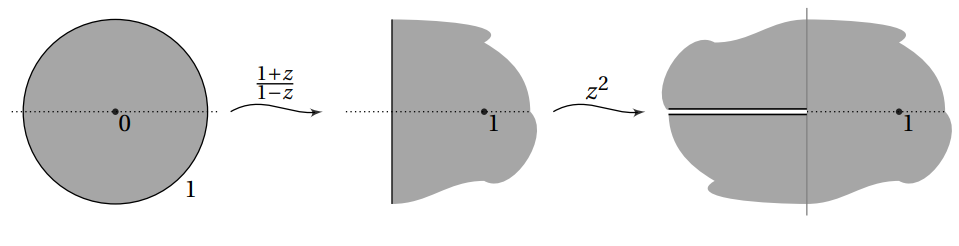
\includegraphics[width=0.8\textwidth]{imagenes/ej4.png}
    \end{align*}
    \item El disco unidad es conformemente equivalente al sector $S_{\alpha} = \{ re^{i\theta} : r > 0, |\theta| < \alpha \}$ de apertura $2\alpha$ ($\alpha \in (0,\pi]$) mediante la aplicación $f_{\alpha}(z) = \left(\frac{1 + z}{1-z} \right)^{\frac{2}{\pi}\alpha}$ y donde se usa la rama principal de la potencia.
    \begin{align*}
        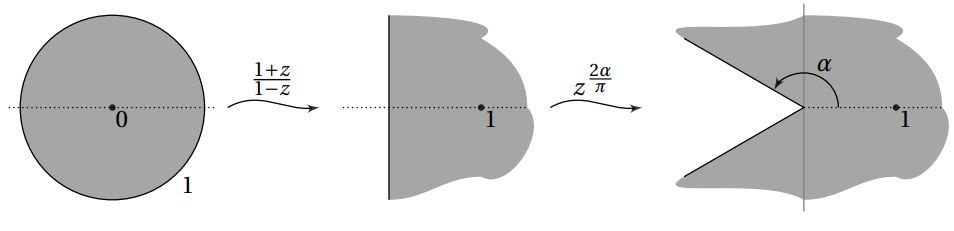
\includegraphics[width=0.8\textwidth]{imagenes/ej5.png}
    \end{align*}
    \item El disco unidad es conformemente equivalente a la banda horizontal $B_{h} = \{ \im |z| < h \}$ de altura $2h$ ($h > 0$), mediante la aplicación $f(z) = \frac{2h}{\pi}\logp\left( \frac{1+z}{1-z}\right)$
    \begin{align*}
        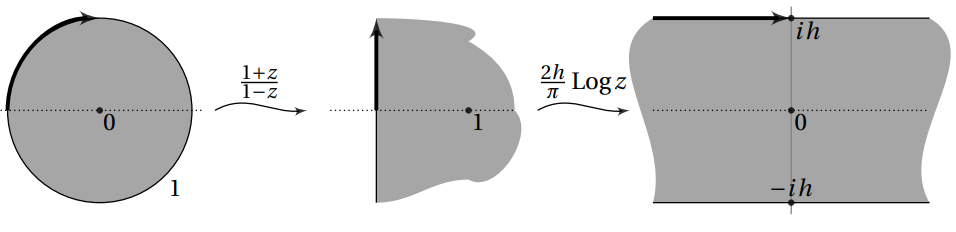
\includegraphics[width=0.8\textwidth]{imagenes/ej6.png}
    \end{align*}
    \item El disco unidad es conformemente equivalente a $\mathbb{H} \backslash [0,1]$, mediante la secuencia de aplicaciones
    \begin{align*}
        &\mathbb{D} \xrightarrow{} \com \backslash (-\infty,0] \xrightarrow{} \com \backslash (-\infty,1] \xrightarrow{} \mathbb{H} \backslash [0,1] \\
        &z \longmapsto \left(\frac{1 + z}{1-z} \right)^2 \longmapsto \bullet + 1 \longmapsto \sqrt{\bullet}
    \end{align*}
    donde nuevamente se ha usado la rama principal de la raíz cuadrada.
    \begin{align*}
        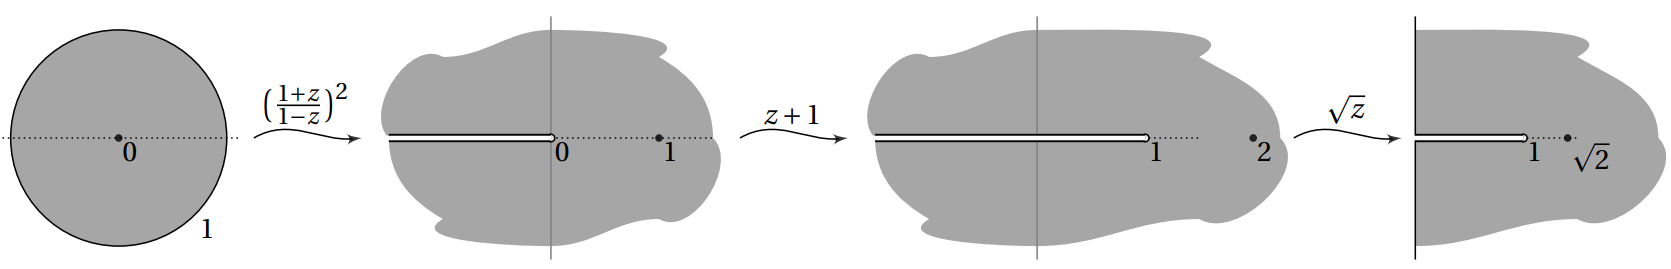
\includegraphics[width=1\textwidth]{imagenes/ej7.png}
    \end{align*}
    \item El disco unidad es conformemente equivalente a $\mathbb{D} \backslash [-1,0]$, usando la aplicación $\sqrt{\left( \frac{1+z}{1-z}\right)^2 + 1}$, $z \in \mathbb{D}$ y luego la inversa de la aplicación de Cayley, $\frac{w-1}{w+1}$, $w \in \mathbb{H}$. Así, una aplicación conforme entre $\mathbb{D}$ y $\mathbb{D} \backslash [-1,0]$ es
    \begin{align*}
        f(z) = \frac{\sqrt{\left( \frac{1+z}{1-z}\right)^2 + 1} -1}{\sqrt{\left( \frac{1+z}{1-z}\right)^2 + 1} + 1}
    \end{align*}
    donde $z \in \mathbb{D}$.
    \begin{align*}
        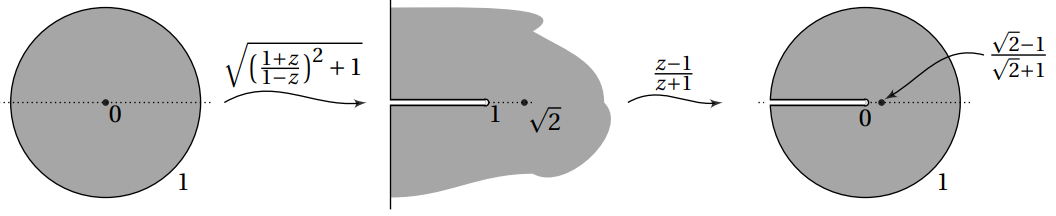
\includegraphics[width=0.8\textwidth]{imagenes/ej8.png}
    \end{align*}
    \item El disco unidad es conformemente equivalente a $\mathbb{D} \backslash \overline{\Delta\left( \frac{1}{2}, \frac{1}{2}\right)}$. La secuencia de aplicaciones sería así
    \begin{align*}
        &\mathbb{D} \xrightarrow{} \mathbb{H} \xrightarrow{} \{  0 < \im z < 1\} \xrightarrow{} \{  0 < \re z < 1\} \xrightarrow{} \overline{\Delta\left( \frac{1}{2}, \frac{1}{2}\right)} \\
         &z \longmapsto \frac{1+z}{1-z} \longmapsto \frac{1}{\pi} \logp(\bullet) + \frac{i}{2} \longmapsto i(\bullet) + 1 \longmapsto\frac{\bullet - 1}{\bullet +1}
    \end{align*}
    \begin{align*}
        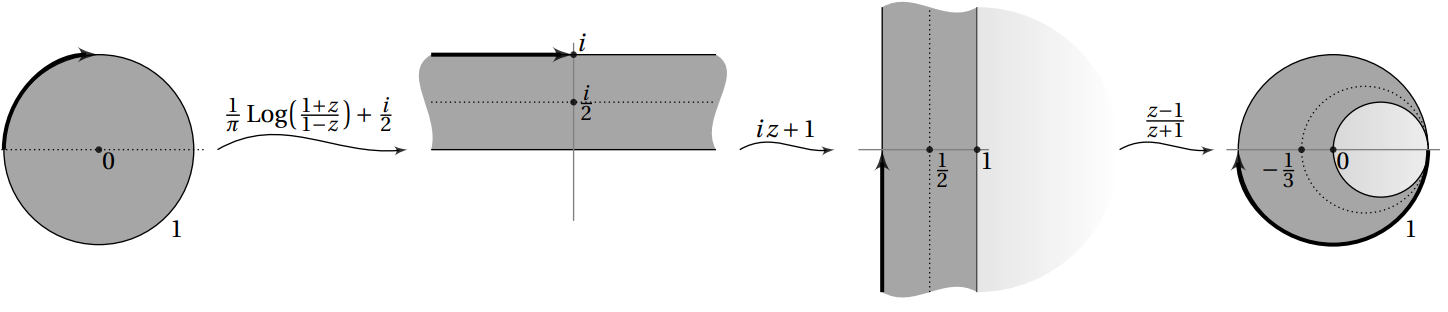
\includegraphics[width=1\textwidth]{imagenes/ej9.png}
    \end{align*}
\end{enumerate}
\end{ejemplo}